
\documentclass[12pt]{siamart}
\usepackage{geometry} % see geometry.pdf on how to lay out the page. There's lots.
\usepackage{bm}
\usepackage{booktabs}
\geometry{a4paper} % or letter or a5paper or ... etc
% \geometry{landscape} % rotated page geometry
\usepackage{algorithm,algorithmic,amssymb,amsmath,letltxmacro}

% See the ``Article customise'' template for come common customisations

\newcommand{\TheTitle}{Runaway electron generation with High-performance, structure preserving discretizations Fokker-Planck-Landau} 
\newcommand{\HTitle}{Runaway Electron Generation with High-performance Fokker-Planck-Landau} 
\newcommand{\TheAuthors}{M. F. Adams, Dylan Brennan, M. G. Knepley}
\newcommand{\Order}[1]{\ensuremath{\mathcal{O}(#1)}}    % big O notation

% Sets running headers as well as PDF title and authors
\headers{\HTitle}{\TheAuthors}

% Title. If the supplement option is on, then "Supplementary Material"
% is automatically inserted before the title.
\title{{\TheTitle}}

% Authors: full names plus addresses.
\author{
  Mark F. Adams\thanks{Lawrence Berkeley National Laboratory, Berkeley CA, USA (\email{mfadams@lbl.gov})}
 \and
 Dylan Brennan \thanks{Princeton University, Princeton NJ, USA}
 \and
  Matthew G. Knepley\thanks{ University at Buffalo, Buffalo NY, USA}
}

%%% BEGIN DOCUMENT
\begin{document}

\date{}

\maketitle

\begin{abstract}
Runaway electron (RE) events are catastrophic to tokamak experimental reactors and pose an existential threat to the development of commercial fusion reactors.
We seek to understand the generation of ``seed" electrons, which are the precursors of REs, with accurate velocity space models using fully conserving, structure preserving, discretizations of the Fokker-Planck collision operator in Landau form.
We continue the development of a high-performance implementation of these discretizations with verification studies and the extension of earlier work on vectorization to general graphical processing units (GPUs).
We investigate seed electron generation as a function of exogenous parameters such as quench rates, heavy ion injection rates from common mitigation strategies, plasma temperature, etc.
\end{abstract}


\begin{keywords}
  Landau collision integral, fusion plasma physics, general graphical processing units, GPUs
\end{keywords}

\section{Introduction}

A runaway electron event can cripple fusion reactor for months and thereby threaten the mission of reactor scale experiments like ITER and the commercial viability of fusion power.
Modeling of the generation of the precursors to runway electrons, seed electrons, is critical in developing mitigation strategies to suppress a catastrophic avalanche of runway electrons.
The Landau form of the Fokker-Planck collision operator is the gold standard for small angle collision dominated plasmas, is fully conservative and admits fully conservative finite element discretizations \cite{Hirvijoki2016,AdamsHirvijokiKnepleyBrownIsaacMills2017}.
The Landau operator, however, exhibits quadric complexity in both the number of mesh points ($N$, integration points) and the number of species ($S$).
We mitigate these costs by first adapting the grid to put mesh resolution where it is needed most, that is to efficiently use our available resources to achieve uniform accuracy without over resolving smooth parts of the distribution functions as discussed in \cite{AdamsHirvijokiKnepleyBrownIsaacMills2017}.
This reduces $N$.
The second strategy to reduce the costs of Landau is to use the fast hardware available for the kernels where the global integrals and the loop with the $\Order{S^2}$ complexity term in our formulation of the algorithm (\S\ref{sec:algo}).



The evolution of the velocity-space density or
distribution function $f$ of each species (ie, electrons and multiple
species of ions in general) in a plasma is modeled with the {\it Vlasov-Maxwell-Landau} system
\begin{equation*}
\frac{df}{dt}\equiv
\frac{\partial f}{\partial t} + \frac{\partial\bm x}{\partial t}
\cdot \nabla_x f+ \frac{\partial\bm v}{\partial t} \cdot \nabla_v f
= \frac{\partial f}{\partial t} + {\bm v} \cdot \nabla_x f+
\frac{e_{\alpha}}{m_{\alpha}}\left( {\bm E} + {\bm v} \times {\bm B} \right) \cdot
\nabla_v f = C + S^M\left(t\right)
\end{equation*}
where $e$ is charge, $m$ mass, ${\bm E} $ electric field, ${\bm B}$
magnetic field, ${\bm x}$ spatial coordinate, ${\bm v}$ velocity
coordinate,  $t$ time and $S^M\left(t\right)$ is an Maxwellian exogenous source with a given temperate $T_{cold}$ and a given number density as a function of time for electrons and a selection ion species (scaled appropriately by a given effective ionization number) \cite{Vlasov1968}.
We ignore configurations space and work only in velocity space and let ${\bm B=0}$.
We use  the Fokker-Planck collision integral in Landau form $C$ \cite{landau1936kinetic}.
With this, the distribution function $f_{\alpha}(\bm{v},t)$ of species $\alpha$ evolves according to

\begin{equation*}
\label{eq:landau1}
\frac{\partial f_{\alpha}}{\partial t} + \frac{e_{\alpha}}{m_{\alpha}} {\bm E} \cdot \nabla f_{\alpha} = 
\sum_{\beta}\nu_{\alpha\beta}\frac{m_o}{m_{\alpha}}\nabla \cdot\int \limits_{\bar\Omega} d\bm{\bar{v}}\;\mathbf{U}(\bm{v},\bm{\bar{v}})\cdot\left(\frac{m_o}{m_{\alpha}}\bar{f}_{\beta}\nabla f_{\alpha} - \frac{m_o}{m_{\beta}}f_{\alpha} \bar \nabla \bar{f}_{\beta}\right) + S^M_\alpha\left(t\right),
\end{equation*}
with derivatives assume to be in velocity space so that we can drop the subscripts.

Here
$\nu_{\alpha\beta}=e_{\alpha}^2e_{\beta}^2\ln\Lambda_{\alpha\beta}/(8\pi m_o^2\varepsilon_0^2)$, $\ln\Lambda$ is the Coulomb logarithm, $m_o$
is an arbitrary reference mass, $\varepsilon_0$ is the vacuum
permittivity, $e$ is electric charge, and $\bm{v}$ is the velocity. Overbar terms are evaluated on the $\bm{\bar{v}}$ grid that covers the domain $\bar\Omega$ of species $\beta$.  The
Landau tensor $\mathbf{U}(\bm{v},\bm{\bar{v}})$ is a scaled projection
matrix defined as
\begin{equation*}
\label{eq:landau_tensor}
\mathbf{U}(\bm{v},\bm{\bar{v}})=\frac{1}{\lvert\bm{v}-\bm{\bar{v}}\rvert^3}\left(\lvert\bm{v}-\bm{\bar{v}}\rvert^2\mathbf{I}-(\bm{v}-\bm{\bar{v}})(\bm{v}-\bm{\bar{v}})\right).
\end{equation*}

\subsection{Normalization with nondimensional variables}

We nondimensionalize our system with a  thermal temperature of electrons $T_e$ and a reference velocity $v_0 = \left ( 8kT_e/m_e\pi \right)^{\frac{1}{2}} $ by defining a velocity coordinate ${\bm x = \bm v / v_0}$.
Normalize the distribution function variable  $\tilde f_{\alpha} = f_{\alpha}v_0^3/n_0$ with a number density $n_0$ (eg, n=$10^{20}$ for a typical fusion plasma).
Define the nondimensional variables to $\tilde t = t/t_0$,  with a reference time scale 
\begin{equation}
\label{eq:ndvars}
t_0 = \frac{8\pi m_o^2\varepsilon_0^2v_0^3}{e^4\ln\Lambda_{ee}n_0}, \quad \text{and define} \quad
\tilde {\bm E} = \frac{ t_0}{v_0} {\bm E}, \quad
\tilde \nu_{\alpha\beta} = \frac{t_0n_0}{v_0^3} \nu_{\alpha\beta}.
\end{equation}
Further, $d\bm{{x}} = v_0^{-3} d\bm{{v}}$, $\mathbf{U}(\bm{x},\bm{\bar{x}}) = v_0\mathbf{U}(\bm{v},\bm{\bar{v}})$  and $\frac{\partial}{\partial \bm x} = v_0\frac{\partial}{\partial \bm v }$.
Note, $\tilde \nu_{ee}=1$.
Any physical velocity space moment is given by $\int \bm{v}^n fd\bm{v}=n_0v_0^{n}\int \bm{x}^nF d\bm{x}$. 
Rewriting the equation in these normalized, dimensionless coordinates results in

\begin{equation*}
\label{eq:landau2}
\frac{\partial \tilde f_{\alpha}}{\partial \tilde t}+  \frac{ e_\alpha}{m_{\alpha}} \tilde{\bm E} \cdot \nabla \tilde f_{\alpha} = 
\sum_{\beta} \tilde \nu_{\alpha\beta}\frac{m_o}{m_{\alpha}}\nabla \cdot\int \limits_{\bar\Omega} d\bm{\bar{x}}\;\mathbf{U}(\bm{x},\bm{\bar{x}})\cdot\left(\frac{m_o}{m_{\alpha}} \tilde {\bar{f}}_{\beta} \nabla \tilde f_{\alpha} - \frac{m_o}{m_{\beta}} \tilde f_{\alpha} {\bar  \nabla} \tilde {\bar {f}}_{\beta}\right)  + S_M\left(t\right).
\end{equation*}

\subsection{Weak Form}

We continue with the weak form of (\ref{eq:ndvars}), assuming nondimensional variables to simplify notation.
We work in gyro-averaged, axisymmetric or cylindrical coordinates $\bm{x} = \left ( r, z \right )$ and assume ${\bm E = E_{z}}$.
According to \cite{Hirvijoki2016,AdamsHirvijokiKnepleyBrownIsaacMills2017}, the weak form of \ref{eq:landau2} for species $\alpha$ is, given a test function $\psi(\bm{x})$,  
\begin{equation}
\label{eq:weak-form}
2\pi \int \limits_{\Omega} d\bm{x} r \psi \cdot \left ( \frac{\partial  f_{\alpha}}{\partial t}  + \left ( 0,  \frac{ e_\alpha}{m_{\alpha}} E_z \right)  \cdot \nabla f_{\alpha}  \right)  = \sum_{\beta}\left(\psi, f_{\alpha}\right)_{\bm{K},\alpha\beta}+\left(\psi,f_{\alpha}\right)_{\mathbf{D},\alpha\beta} + \left(\psi,S^M_\alpha\right) ,
\end{equation}
where $(\cdot,\cdot)_{\Omega}$ is the standard $L^2$ inner product in $\Omega$ and the weighted inner products present the advective and diffusive parts of the Landau collision integral
\begin{align}
\label{eq:K}
\left(\psi, \phi\right)_{\bm{K},\alpha\beta}&=\int \limits_{\Omega}d\bm{x}r\nabla_{v}\psi\cdot {\nu}_{\alpha\beta}\frac{m_o}{m_{\alpha}} \frac{m_o}{m_{\beta}}\bm{K}(f_{\beta},\bm{x})\, \phi,\\
\label{eq:D}
\left(\psi,\phi\right)_{\mathbf{D},\alpha\beta}&=-\int \limits_{\Omega}d\bm{x}r\nabla_{v}\psi\cdot{\nu}_{\alpha\beta}\frac{m_o}{m_{\alpha}}\frac{m_o}{m_{\alpha}}\mathbf{D}(f_{\beta},\bm{x})\cdot\nabla_{v}\phi
\end{align}
with the distribution function of species $\beta$, $f_{\beta}$, the vector $\bm{K}$ and the tensor $\mathbf{D}$ are defined as
%\begin{equation}
% \begin{align*}
%   \bm{K}_{\beta}(\bm{x})&=\int \limits_{\Omega_{\beta}}d\bm{\bar{x}}\;\mathbf{U_K}(\bm{x},\bm{\bar{x}})\cdot\bar{\nabla}_{\bar{v}}\bar{\lambda}_{\beta}(\bm{\bar{x}}), \\
% \end{align*}
\begin{align}
\label{eq:fric_coef}
  \bm{K}(f,\bm{x})&=\int \limits_{\bar\Omega}d\bm{\bar{v}}\bar r\;\mathbf{U}^K(\bm{x},\bm{\bar{v}})\cdot\bar{\nabla}_{\bar{v}}f(\bm{\bar{v}}), \\
\label{eq:diff_coef}
  \mathbf{D}(f,\bm{x})&=\int
  \limits_{\bar\Omega}d\bm{\bar{v}}\bar r\;\mathbf{U}^D(\bm{x},\bm{\bar{v}})f(\bm{\bar{v}}).
\end{align}
Note, these Landau tensors in cylindrical coordinates is quite a bit more complex (about 165 flops including 4 transcendental functions).
See Hirvijoki and Adams for the definitions of $\mathbf{U}^K$ and $\mathbf{U}^D$ \cite{Hirvijoki2016}.

\subsection{Maxwellians}
Distribution functions are initialized, including sources in the model, with Maxwellian distributions in normalized units.
The particle density is defined according to 
$$ f_\alpha\left ( {\bm x}, T_\alpha \right ) = n_\alpha \int_{R^3} dx^3 \left(\frac{m_\alpha v_0^2}{2\pi kT_\alpha}\right)^{3/2}\exp [- m_\alpha v_0^2{\bm x}^2/(2kT_\alpha)] .$$
Defining $\theta=2kT_\alpha/m_\alpha v_0^2$, we thus find that the probability density 
 for finding the particle within the interval in a box d$x^3$ around x is, given number density $n$ 
 
 \begin{equation*}
\label{eq:maxwellian}
  \  f_\alpha \left (x;\theta \right )= \ n_\alpha\left(\frac{1}{\pi\theta}\right)^{3/2} \exp [ -{\bm x}^2/\theta ]
\end{equation*}

\section{Code structure and verification}
We use the fully non-linear multi-species conservative finite element discretization of the Landau integral \cite{Hirvijoki2016,AdamsHirvijokiKnepleyBrownIsaacMills2017} with the PETSc numerical library \cite{petsc-web-page,petsc-user-ref}. 
PETSc provides finite element support, mesh management and non-conforming mesh adaptivity with an interface to the {\it p4est} library
\cite{Stadler1033,DBLP:journals/siamsc/IsaacBWG15,Rudi:2015:EIS:2807591.2807675}.
We use standard, high order tensor product finite elements and a single grid with a degree-of-freedom for each species at each grid point.
Figure \ref{fig:grids} shows the initial conditions for a 4 keV ion-deuterium plasma with a typical grid adapted to for stationary verification test.
\begin{figure}[htbp]
\begin{center}
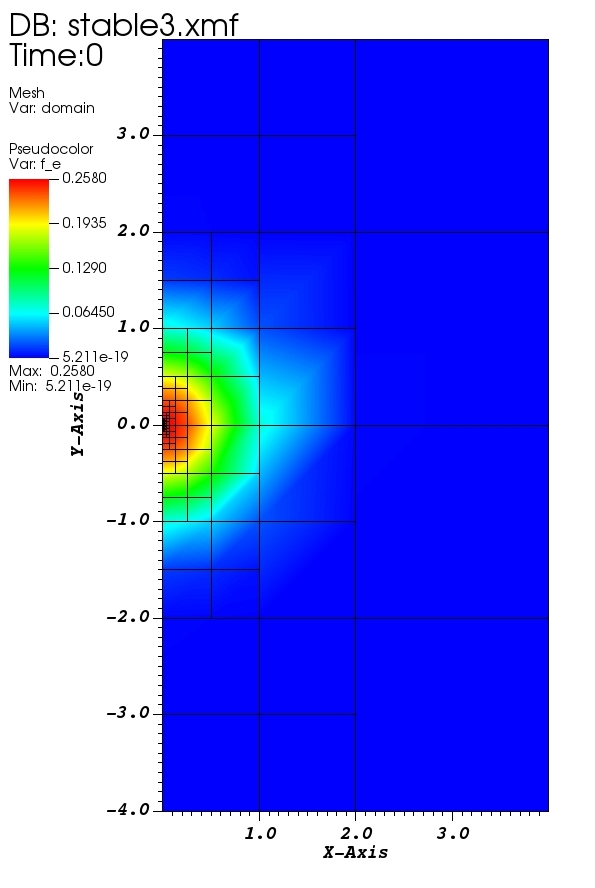
\includegraphics[width=.34\linewidth]{AMR0003.jpeg}
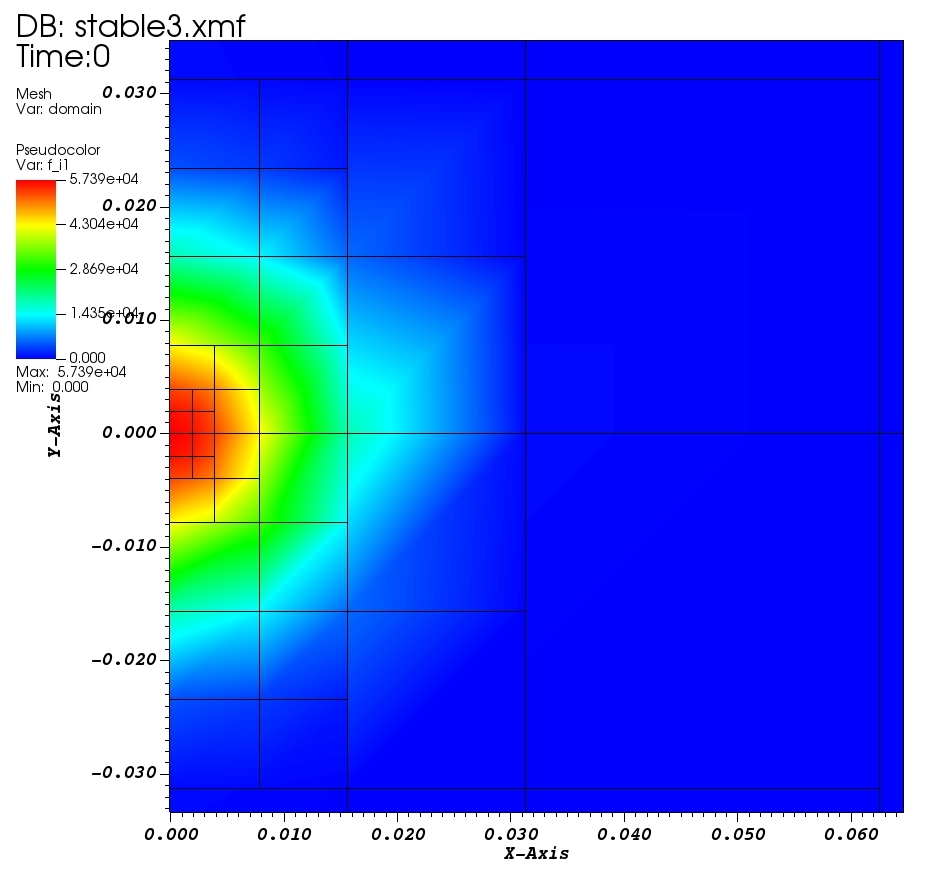
\includegraphics[width=.55\linewidth]{AMR0002.jpeg}
\caption{Electron distribution function on whole domain of electron-deuterium plasma (left), ion distribution function detail (note the two orders of difference in scale) (right)}
\label{fig:grids}
\end{center}
\end{figure}
Note, This visualization uses linear interpolation (by subdividing each square into two triangles), whereas the finite element spaces are higher order tensor product polynomials and are hence much more accurate and symmetric about $x_z=0$.

\subsection{Verification of stationary Maxwellians}
Maxwellians are eigenfunctions of the Landau operator.
Multiple species with the same thermal temperature are similarly eigenfunctions of the multi-species Landau operator.
Alas, these discrete finite functions are not eigenvectors of the our discretized operator and, as has been observed by others \cite{Hager2016}, they can not be exactly preserved, however our discretizations do converge to a stable operator.
We demonstrate this with an electron-deuterium plasma with  $T_i=T_e=4 keV$, the domain and mesh in Figure \ref{fig:grids}. 
We use $n_0=10^{20}$, $\ n_i = \ n_e = 1$, and run for time $\ t = 1.0$ second ($t_0 = 4.6\times 10^{-5}$).
We refine in the polynomial degree of the finite elements, using quartic (Q2), cubic (Q3), quartic (Q4) and quintic (Q5) elements.

Figure \ref{fig:stable} shows a L2-norm of the difference between the finite element solution and the exact initial Maxwellian function, normalized with the L2-norm of the Maxwellian, which includes the finite element discretization error.
We use the adaptive time stepper, a first order Backward Euler represented as an ARK IMEX scheme with extrapolation as error estimator \cite{abhyankar2018petscts}.
We use an exact, LU, solver within a Newton non-linear solver with tolerances of $10^{-8}$ and relative tolerance of $10^{-6}$ in the time integrator.
The mesh has 170 elements, which results in 1,530-6,120 integration points total with Q2-Q5 elements.
\begin{figure}[htbp]
\begin{center}
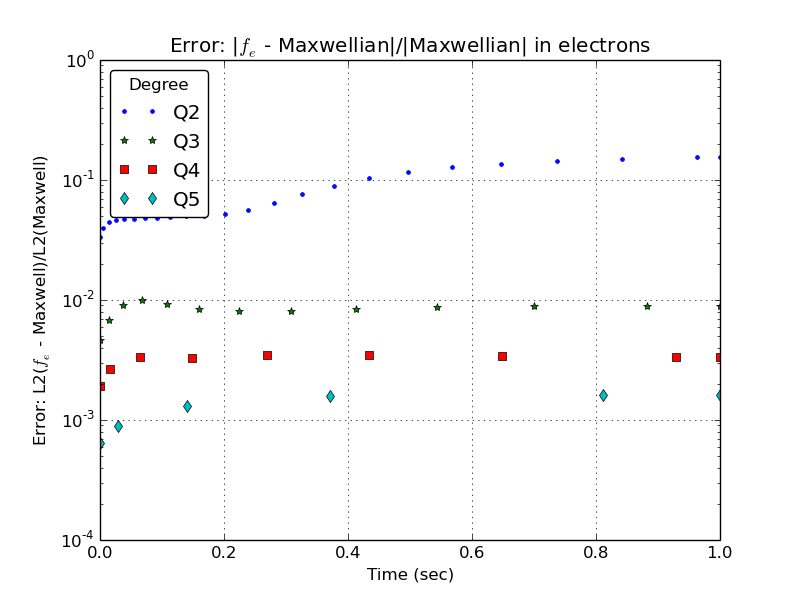
\includegraphics[width=.4\linewidth]{e_L2error.png}
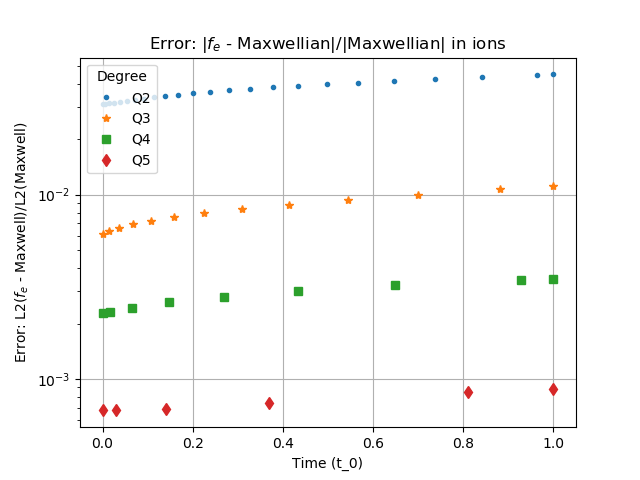
\includegraphics[width=.4\linewidth]{i_L2error.png}
\caption{L2 norm of deviation of solution from the exact initial Maxwellian at every 10 time steps, as well as the last time step, of electrons (left) and deuterium ions (right)}
\label{fig:stable}
\end{center}
\end{figure}

This data shows that the solution deviates from the initial, ideally stable, condition with an error of approximately the same scale as the discretization error, and these errors are reduced with increased order of accuracy, indicating that the discretization is converging to a stable solution.
Additionally, Figure \ref{fig:stable} indicates the time steps taken by the adaptive time step method, outputting data every 10 time steps (and the last step); we observe the larger time steps allowed by high-order methods.
Figure \ref{fig:error} shows the difference of the finite element solution and its initial conditions, with Q4 elements, at $\ t = 0.2$.
\begin{figure}[htbp]
\begin{center}
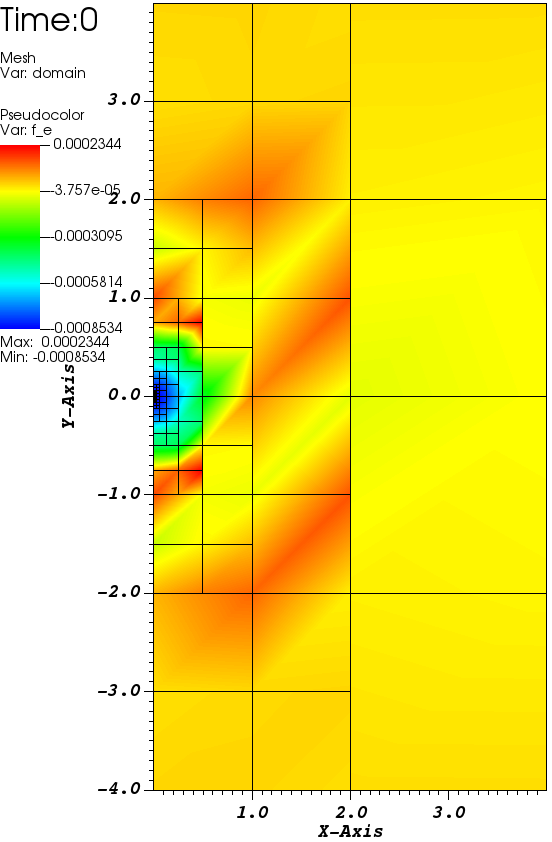
\includegraphics[width=.22\linewidth]{e_error.png}
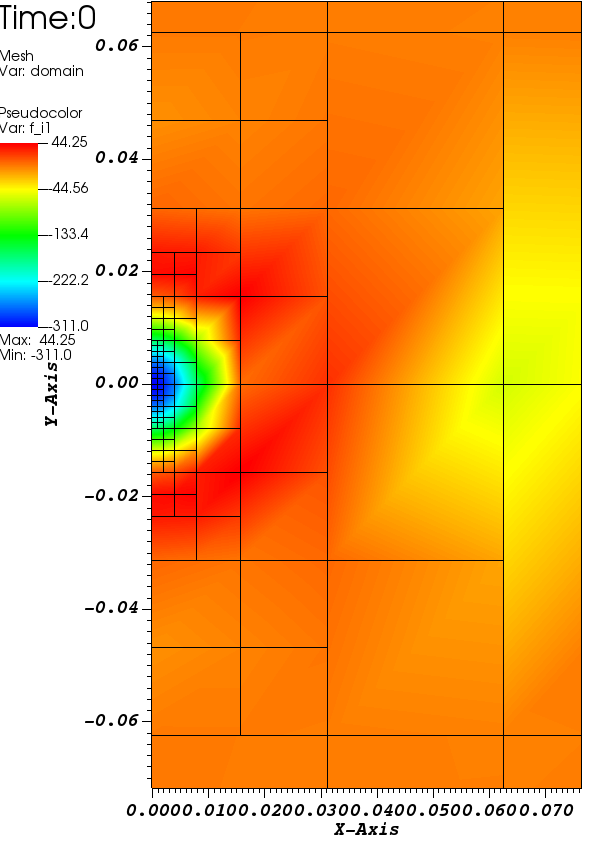
\includegraphics[width=.24\linewidth]{i_error.png}
\caption{Example of discrete error, the difference between the solution and the initial Maxwellian function of electrons (left) and ions (right)}
\label{fig:error}
\end{center}
\end{figure}

\subsection{Verification with Spitzer resistivity}

Spitzer resistivity is a classical model of electrical resistivity commonly used in plasma physics, based upon electron-ion collisions \cite{Spitzer1950,Spitzer1953}. The transverse Spitzer resistivity is given by:

$${ \eta _{\perp }={\frac {4{\sqrt {2\pi }}}{3}}{\frac {Ze^{2}m_{e}^{1/2}\ln \Lambda }{\left(4\pi \varepsilon _{0}\right)^{2}\left(k_{\text{B}}T_{e}\right)^{3/2}}},}$$

and the parallel resistivity is given by $ {\eta_{z} = \eta _{\perp} F(Z)} $, with

$${ F(Z)={\frac {1+1.198Z+0.222Z^{2}}{1+2.966Z+0.753Z^{2}}}}$$.

We verify our code by applying and electric field ($E_{z}=10^{-1} N/C$), computing a finite element integral of the current.
The velocity space model can create a current with an applied electric field.
This parallel current can be computed with $ J_z =\sum_{\alpha} \int \limits_{\Omega}d\bm{x} q_\alpha x_{z} f_\alpha(\bm{{x}}), $ and the effective resistivity of the model is $\eta_c = E_{z}/J_{z}$.
$J_{z}$ asymptotes to a constant, within a range of several decades of $E_{z}$; we run the code until the changes in $J_{z}$ are negligible.
We have informally verified that the ratio of our $\eta = E/J$ to the Spitzer $\eta_z$  is not sensitive to any parameters such as temperature and solver parameters.
Figure \ref{fig:z} plot the value of  $\eta = E/J$ to the Spitzer $\eta_z$ as a function of the ionization of the ions ($Z$).
\begin{figure}[htbp]
\begin{center}
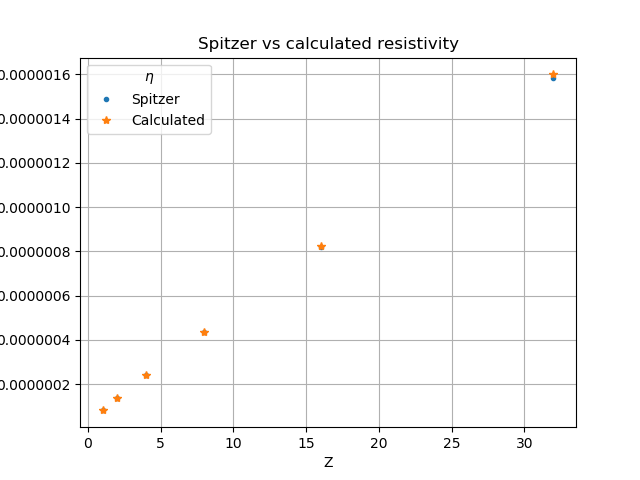
\includegraphics[width=.9\linewidth]{spitzer_calc_eta_Z.png}
\caption{Calculate $\eta = E/J$ and the Spitzer $\eta_z$ as a function of $Z$}
\label{fig:z}
\end{center}
\end{figure}
This data was run with a highly resolved mesh, 512 cells and Q5 elements resulting in 18,468 integration points, and is probably not fully resolved.
We do see with this data that the calculated $\eta$ is within $1\%$ of the Spitzer value.


\section{Use of graphical processing units (GPUs)}

Our approach to utilizing GPUs builds on our approach to vectorizing the code for Intel's Knights Landing processor \cite{AdamsHirvijokiKnepleyBrownIsaacMills2017}.
Algorithm \ref{fig:algo0} shows high level pseudo-code for construction the
Landau Jacobian matrix, with $|G_\alpha|$ cells in the set $G_\alpha$ for species $\alpha$, $N_q$
quadrature points in each element, distribution functions $f$, $S$
species, and weights $w_{q_j} = |J\left(q_j\right)| \cdot q_j.weight
\cdot q_j.r$, where $q_j.r$ is the axisymmetric term of the element
Jacobian, $q_j.weight$ is the quadrature weight of $q_j$, and
$J\left(q_j\right)$ is the element Jacobian at point $q_j$.
\begin{algorithm}[h!]
\begin{algorithmic}[100]
\FOR{$\alpha=1:S$}
\FORALL{cells $i \in G_\alpha$}
\FORALL{quadrature points $q_i \in i$}
\FOR{$\beta=1:S$}
\FORALL{cells $j \in G_\beta$}
\FORALL{quadrature points $q_j \in j$}
%\end{algorithmic} 
%\begin{algorithmic}[100]
\STATE{$\mathbf{U}  \leftarrow \mathbf{LandauTensor}\left(q_i.r,q_i.z,q_j.r,q_j.z\right)$  } 
\STATE{$\mathbf{K} \leftarrow \hat{\nu}_{\alpha\beta}\frac{m_o}{m_{\alpha}}\frac{m_o}{m_{\beta}} \mathbf{U} \cdot \nabla f_\beta\left( q_j \right) w_{q_j} $}
\STATE{$\mathbf{D} \leftarrow - \hat{\nu}_{\alpha\beta}\frac{m_o}{m_{\alpha}}\frac{m_o}{m_{\alpha}} \mathbf{U} f_\beta\left( q_j \right) w_{q_j} $}
\STATE{$\mathbf{C} \leftarrow FiniteElementAssemble\left(\mathbf{C}, w_{q_i} , \mathbf{K},  \mathbf{D} \right)$}
\ENDFOR
\ENDFOR
\ENDFOR
\ENDFOR
\ENDFOR
\ENDFOR
\end{algorithmic} 
\caption{Pseudo-code to compute Landau Jacobian $\mathbf{C}$ with state $f$}
\label{fig:algo0}
\end{algorithm}
The six loops of Algorithm \ref{fig:algo0} can be processed in many orders, and blocked, giving different data access patterns, which is
critical in optimizing performance.
We use one grid for all species, which has advantages and disadvantages \cite{AdamsHirvijokiKnepleyBrownIsaacMills2017}, and results in only one set of cells $G$.
Our kernel of interest is the construction of the tensor and vector in (\ref{eq:K}) and (\ref{eq:D}).
To optimized the processing in the kernel we build a flat array(s) of the data required in the kernel ($\bm x$, $w$, $f_{\alpha}$,  $\frac{\partial f_{\alpha}}{\partial \bm x}$,  $f_{\beta}$,  $\frac{\partial f_{\beta}}{\partial \bm x}, ... $) for all integration points ($N = | G | \cdot N_q$).

Algorithm \ref{fig:algo2} shows the pseudo-code for the CUDA kernel for constructing the Landau collision integral element matrix using standard finite element processes including finite element tabulation at integration points $q_i$, $\mathcal{B}\left(q_i\right),  \mathcal{D}\left(q_i\right)$, and element Jacobian $\mathcal{J}\left(q_i\right)$.
\begin{algorithm}[h!]
\begin{algorithmic}[100]
\STATE{$ N_q \leftarrow blockDim.x$} 
\STATE{$ my\_elem \leftarrow blockIdx.x $} 
\STATE{$ my\_qi  \leftarrow  threadIdx.x$} 
\STATE{$ my\_sub\_blk =  threadIdx.y$}
\STATE{$i \leftarrow my\_qi + my\_elem * N_q $} \COMMENT{global integration point for this thread}
\STATE{$nip  \leftarrow  gridDim.x \cdot N_q $} \COMMENT{global number of integration points}
\STATE{$sz \leftarrow nip/n\_sub\_blocks \quad + \quad !!(nip\%n\_sub\_blocks)$} 
\STATE{$ip\_start \leftarrow my\_sub\_blk*sz$} 
\STATE{$ip\_end \leftarrow (my\_sub\_blk+1)*sz \quad > \quad nip \quad ? \quad nip \quad : \quad (my\_sub\_blk+1)*sz$} 
\FOR[fused inner element and quadrature loop]{$j=ip\_start:ip\_end$}
\STATE{$\left[\mathbf{U_K}, \mathbf{U_D} \right]  \leftarrow \mathbf{LandauTensor}\left(q_i.r,q_i.z,r[j],z[j]\right)$  }
\FOR{$\alpha=0:S$}
\FOR{$\beta=0:S$}
\STATE{$\mathbf{K}\left[my\_qi \right]  \left[my\_sub\_blk \right] \left[{\alpha}\right] \leftarrow \mathbf{K}\left[my\_qi \right]  \left[my\_sub\_blk \right] \left[{\alpha}\right] + \hat{\nu}_{\alpha\beta}\frac{m_o}{m_{\alpha}}\frac{m_o}{m_{\beta}} \mathbf{U_K} \cdot df[\beta][j] w[j]$}
\STATE{$\mathbf{D}\left[my\_qi \right]  \left[my\_sub\_blk \right] \left[{\alpha}\right] \leftarrow \mathbf{D}\left[my\_qi \right]  \left[my\_sub\_blk \right] \left[{\alpha}\right] - \hat{\nu}_{\alpha\beta}\frac{m_o}{m_{\alpha}}\frac{m_o}{m_{\alpha}} \mathbf{U_D} f[\beta][j] w[j]$}
\ENDFOR
\ENDFOR
\ENDFOR
\FOR{$\alpha=0:S$}
\STATE{$\mathbf{G2}\left[my\_qi  \right] \left[my\_sub\_blk \right] \left[{\alpha}\right]  \leftarrow \mathcal{J}\left(q_i\right)^{-T} \mathbf{K}\left[my\_qi \right]  \left[my\_sub\_blk \right] \left[{\alpha}\right] w[i]$} 
\STATE{$\mathbf{G3}\left[my\_qi  \right] \left[my\_sub\_blk \right] \left[{\alpha}\right] \leftarrow \mathcal{J}\left(q_i\right)^{-T} \mathbf{D}\left[my\_qi \right]  \left[my\_sub\_blk \right] \left[{\alpha}\right] \mathcal{J}\left(q_i\right)^{-1} w[i]$}
\ENDFOR
\IF[One sub-block in each integration point sums up sub-blocks]{$my\_sub\_blk = 0$}
\FOR{$b=1:n\_sub\_blocks$}
\FOR{$\alpha=0:S$}
\STATE{$\mathbf{G2}\left[my\_qi  \right] \left[ 0 \right] \left[{\alpha}\right]  \leftarrow      \mathbf{G2}\left[my\_qi  \right] \left[ 0 \right] \left[{\alpha}\right]  +   \mathbf{G2}\left[my\_qi  \right] \left[b\right]  \left[ \alpha \right] $}
\STATE{$\mathbf{G3}\left[my\_qi  \right] \left[ 0 \right] \left[{\alpha}\right]  \leftarrow      \mathbf{G3}\left[my\_qi  \right] \left[ 0 \right] \left[{\alpha}\right]  +   \mathbf{G3}\left[my\_qi  \right] \left[b\right]  \left[ \alpha \right] $}
\ENDFOR
\ENDFOR
\ENDIF
\IF[On master thread in each block]{$threadIdx.x +  threadIdx.y = 0$}
%\STATE{$\mathbf{ElemMats} \left[blockID\right] \leftarrow 0$} \COMMENT{On master thread in each block}
\FOR[Project point value to vertices of cell $i$ with standard FE process]{$i=1:N_q$}
\STATE{$\mathbf{A}\left[my\_elem\right] \leftarrow  \mathbf{A}\left[my\_elem\right]  +  \mathcal{D^T}\left(q_i\right) \mathbf{G3}\left[ i \right]  \left[ 0 \right]  \left[ : \right]  \mathcal{D}\left(q_i\right)  +  \mathcal{D^T}\left(q_i\right) \mathbf{G2}\left[ i \right]  \left[ 0 \right]  \left[ : \right]  \mathcal{B}\left(q_i\right)$}
\ENDFOR
\ENDIF
%\FORALL[CPU: Assemble element matrices into global Jacobian]{cells $c \in G$}
%\STATE{$\mathbf{C} \leftarrow \mathbf{C} + GlobalAssemble\left(c, \mathbf{ElemMats}\left[c\right]  \right)$}
%\ENDFOR
\end{algorithmic} 
\caption{CUDA kernel; input: $r$, $z$, $w$, $f$, $df$;
  output: element matrix $\mathbf{A}$ }
\label{fig:algo2}
\end{algorithm}
One element is placed in each CUDA thread block and there is a 2D array of threads $(N_q, number\_sub\_threads)$ per block, with $number\_sub\_threads$ being  a runtime parameter for the number of threads to use within each integration point.
These element matrices are then assembled on the CPU into the global Jacobian.
%This algorithm is designed to minimized data movement by computing the Landau tensors on the fly, they can be precomputed, and it exploits a single mesh by hoisting the tensor kernel outside of the two inner loops over species.
This loop ordering puts the Landau tensor, some of the $\Order{S^2}$ complexity terms, the inner finite element integral and the Jacobian coordinate transformation into a GPU kernel.
A summation of the each threads $G2$ and $G2$ is accumulated by one thread at each integration point and the finite element projection to vertices, from each integration point, is processed by one thread in each thread block.

Algorithm \ref{fig:algos}
shows the initialization of the vectors $r$, $z$, $w$, $f$, and the
gradient vectors $df$, with $|G|$ cells in the set
$G$, $S$ species, and weights $w_{q_i}$ at each quadrature point $i$.
Each quadrature point $q_i$ has a 2D coordinate ($q_i.r$,$q_i.z$).
\begin{algorithm}[h!]
\begin{algorithmic}[100]
\FORALL{cells $i \in G$}
\FORALL{quadrature points $q_i \in i$}
\STATE{$r.append(q_i.r)$}
\STATE{$z.append(q_i.z)$}
\STATE{$w.append( |J\left(q_i\right)| \cdot q_j.weight \cdot q_i.r$)}
\FOR{$\alpha=1:S$}
\STATE{$f[\alpha].append(f_\alpha(q_i) $)}
\STATE{$df[\alpha].append(\nabla f_\alpha(q_i) $)}
\ENDFOR
\ENDFOR
\ENDFOR
\end{algorithmic} 
\caption{Initialization of vectors $r$, $z$, $w$, $f$, and $df$ with state $f$}
\label{fig:algos}
\end{algorithm}

\section{Performance}
We use a node with 2 IBM POWER9 sockets and 6 Nvidia Tesla V100 GPUs / node, using 1 MPI process with one GPU.
This test problem is similar to the problems used for verification, with 62 cells, Q3 elements (992 integration points).
Figure \ref{fig:perf} show the time for the construction of the Jacobian matrix, the GPU kernel, and the CPU matrix assemble and solve.
\begin{figure}[htbp]
\begin{center}
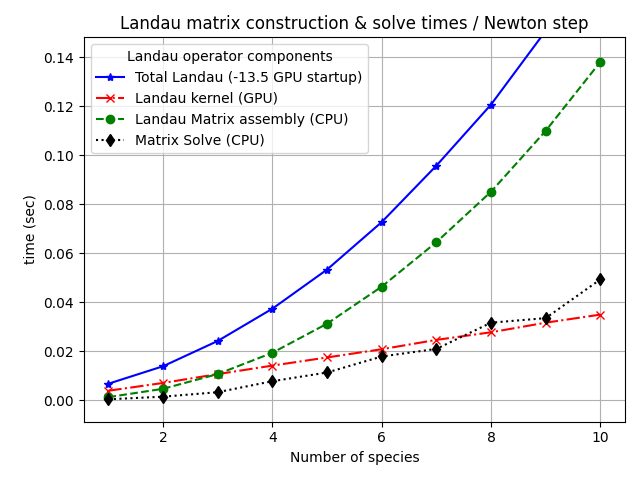
\includegraphics[width=.6\linewidth]{./PPT/landau_time_species.png}
\caption{Times (sec) for Landau Jacobian construction.}
\label{fig:perf}
\end{center}
\end{figure}
We observe that the times increase linearly with number of species, in the GPU kernel, however the serial matrix assemble times increase quadratically.
The matrix assembly has not been parallelized.
One can color elements and assemble them in parallel, or use a local domain decomposition and use standard parallel assembly methods.
If we assume that we can color a 2D block structured AMR grid with 8 colors, then we could expect a speed up of about 8 for this problem with 62 cells.
This should be enough to keep the matrix assembly subdominant.

\section{Seed runaway electron generation}

Runaway electrons (REs) are formed, to put it simply, when a disruption or mitigation mechanism causes a thermal quench, flattening the density profile in velocity space.
This reduces the collisional drag on fast electrons in the tail of the distribution.
A parallel electric field can accelerate these electrons whereby they see even less drag from the body of the population.
These electrons can accelerate indefinitely, subject to relativistic effects and radiative effects.
Relatively small populations of electrons can be accelerated to relativistic velocities and carry significant energy.
If these REs stay on a closed flux surface they can dissipate slowly as the plasma current dissipates.
If, however, field lines become stochastic, as in a disruption, beams of REs can hit the wall of the containment vessel and cause significant damage.
REs are considered to be the primary threat to the mission of ITER and thus it is important to understand their behavior so that the can be avoided or effective mitigations strategies can be designed.

We use our highly accurate, fully nonlinear Landau collisional model to help to understand RE generation and focus on the seed electron generation, the generation of populations that are the beginnings of a runaway event.
Our model uses an exogenous source of impurities $S\left(t\right)$ to cause a thermal quench in the plasma.
This source adds a term, $\left(\psi,S_{\alpha}\right)$, to the right hand side of  (\ref{eq:weak-form}) at each time step.
This is a crude model of a mitigation strategy where impurity pellets are injected into the plasma.
Note, REs are generated from a thermal quench caused by plasma disruptions, generally.
Impurity injection causes a thermal quench also and is easier to model with a $0D$ model.
We thus us a model that looks like a mitigation strategy, for convenience, to generate a thermal quench and generate REs.
We assume that the source is fully ionized, generating a number density $n_e$ for electrons and $n_i$ for one ion species with a Maxwellian distribution and temperature of given $T_{cold}$ (eg, 5 ev).
Thus a rate, $dn/dt$ is provided at each time step, a Maxwellian distribution for electrons is then created with $S_e = dn_e/dt =  dn/dt$, one for ions is created with $S_i = dn_i/dt =  Z dn/dt$, were $Z$ is the effective ionization of the ions, and both have a provide temperature $T_{cold}$.
$\left(\psi,S_{\alpha}\right) = M S_\alpha$ is added as a source term to the discrete equations.
$M$ is the finite element mass matrix in cylindrical coordinates.

We consider the relationship between plasma temperature and quench rate in the generation of REs.
We apply a constant electric field in the parallel direction of magnitude $? E_c$, where $E_c$ is the Connor-Hastie electric field $E_c =n_e e^3\ln \Lambda / \left (4 \pi \epsilon_0^2 m_e c^2\right)$ \cite{Connor1975}.
A source term function ....

\section{Conclusion}

\section{Acknowledgments}

 This work was partially funded from the DOE contract number
DE-AC02-09-CH11466.  This research used resources of the National
Energy Research Scientific Computing Center, a DOE Office of Science
User Facility supported by the Office of Science of the
U.S. Department of Energy under Contract No. DE-AC02-05CH11231.

\bibliographystyle{unsrt}
\bibliography{the}

\end{document}